\documentclass[a4paper,10pt]{article}
\usepackage[utf8]{inputenc}
\usepackage{graphicx}
\usepackage{caption}
\usepackage{subcaption}
\title{IN4320 Machine Learning Exercise 1}
\author{Xiang Teng (4574060)}

\begin{document}

\maketitle


\section{Question1}
\begin{itemize}
    \item Figure \ref{fig:loss function} shows the drawing of the loss function as a function of $m_+$
        \begin{figure}[h]
        \centering
            \includegraphics[width=8cm]{1_a_v2.png}
                \caption{the drawing of the loss function as a function of $m_+$ for all $\lambda \in $ {0,2,4,6}}
                \label{fig:loss function}
        \end{figure}
    \item Derive the minimizer and their minimum values
    \begin{itemize}
        \item The minimizer and their minimum values:
        \begin{enumerate}
            \item $\lambda$ = 0, min = 2 with minimizer (0,2);
            \item $\lambda$ = 2, min = 3.5 with minimizer (0.5,3.5);
            \item $\lambda$ = 4, min = 4 with minimizer (1, 4);
            \item $\lambda$ = 6, min = 4 with minimizer (1, 4);
    \end{enumerate}
        \item the points where their derivative equals to 0 (or around 0) are:
        \begin{enumerate}
            \item $\lambda$ = 0, min = 2 with minimizer (0,2);
            \item $\lambda$ = 2, min = 3.5 with minimizer (0.5,3.5);
            \item $\lambda$ = 4, min = 4.0008 with minimizer (0.98, 4.0008);
            \item $\lambda$ = 6, min = 4.0408 with minimizer (0.98, 4.0408); 
        \end{enumerate} 
    \end{itemize}
    
      The related gradients (around 0) are 0, 0, 0.0016 and 0.0416 respectively while $\lambda$ has the value 0, 2, 4 or 6. This concludes that for both methods, The same minimum points are found.
    
\end{itemize}
\newpage
\section{Question2}
\begin{itemize}
    \item a) \\
    The regularizer is trying to enforce the difference between two mean values. If $\lambda$ gets larger and larger, the regularization term will have a dominant position in the loss function. The influence of the data-dependent error decrease. If $\lambda$ is sufficiently large, some of the coefficients $w_j$ are driven to zero, leading to a sparse model in which the corresponding basis functions play no role. Therefore, the problem of over-fitting is solved.
    \item b) \\
    This is the case of $q=1$, it is known as \textit{lasso} in the statistics literature.
    The unregularized error functions ($\lambda = 0 $) has the shape of the circle. multiple circles have the different size but with the same central point. Each circle stands for the points which have the same value in 3-d space
    The regularized error function has the shape of the rotated rectangle. Figure \ref{fig:lasso} shows how the contours of these two basic geometric shapes look like.
        
    \begin{figure}[h]
            \centering
            \begin{subfigure}[b]{0.3\textwidth}
              \includegraphics[width=\textwidth]{lasso.PNG}
                \caption{The contours of the unregularized error function (blue) along with the constraint region for the lasso regularizer $q=1$ }
                \label{fig:lasso}
            \end{subfigure}
            ~ %add desired spacing between images, e. g. ~, \quad, \qquad, \hfill etc. 
              %(or a blank line to force the subfigure onto a new line)
            \begin{subfigure}[b]{0.6\textwidth}
                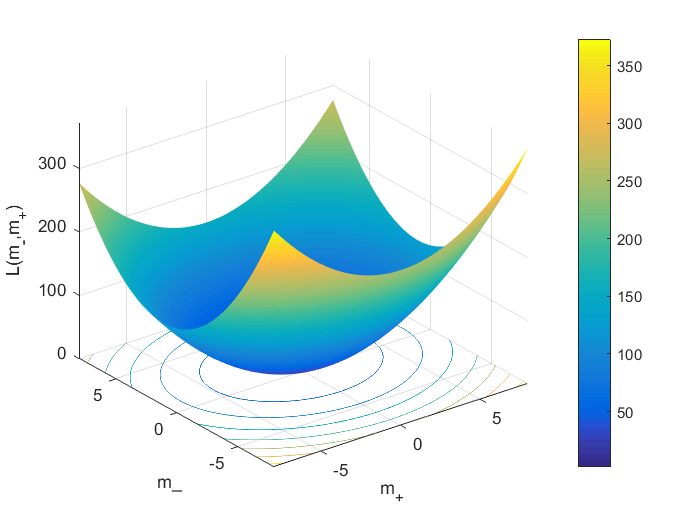
\includegraphics[width=\textwidth]{3d_q2c.png}
                \caption{A given 3d drawing after minimizing L for both $m_\_$ and $m_+$ with $\lambda = 4$. The shape of the contours are the circles lay on the ground plane}
                \label{fig:3d}
            \end{subfigure}
            ~ %add desired spacing between images, e. g. ~, \quad, \qquad, \hfill etc. 
            %(or a blank line to force the subfigure onto a new line)
            \caption{Contours analysis for the regularized loss function}
        \end{figure}
        
    \item c) \\
    If $\lambda$ is sufficiently large, the corresponding basis functions play no role. The loss function now could be written as:
    \begin{equation}
        L(m_\_,m_+) = \lambda||m_\_-m_+||_1
    \end{equation}
    The minimum value is 3.2 and remains constant while $\lambda$ is bigger than 4, the mean values are $m_\_ = 0.6$ and $m_+ = 0.6$.
\end{itemize}
\section{Question3}
    \begin{equation}\label{eq:1}
        L(m_\_,m_{+}) = \sum_{i}^{N}||X_i-m_{y_i}||^2+ \lambda||m_\_-m_+||_1
    \end{equation}

The derivative of equation \ref{eq:1} respect to $m_\_$ and $m_+$ are 
    \begin{equation}
        \frac{\partial L(m_\_,m_+)}{\partial m_\_}=2\sum_{i}^{N}(m_\_-x_i) +\lambda*sign(m_\_-m_+)
    \end{equation}
       \begin{equation}
        \frac{\partial L(m_\_,m_+)}{\partial m_+}=2\sum_{i}^{N}(m_+-x_i) +\lambda*sign(m_+-m_\_)
    \end{equation} 
    respectively.
\begin{itemize}
    \item a)
    Gradient descent is used as the search strategy. Firstly, a random mean value for both $m_\_$ and $m_+$ are picked. And then the derivative of loss function respect to both mean values are calculated. After that, an iteration process is executed based on the following equations:
        \begin{equation}
            m_\_ = m_\_ -\alpha*\frac{\partial F(m_\_,m_+)}{\partial m_\_}
        \end{equation}
        \begin{equation}
            m_+ = m_+ -\alpha*\frac{\partial F(m_\_,m_+)}{\partial m_+}
        \end{equation}
        with $\alpha$ is the learning rate. The iteration stops while the difference between $m_\_$ and $m_+$ is smaller than a certain value.
    \item b) Figure \ref{fig:mean image 0} shows the mean images for both {+, -} class while $\lambda = 0$. And Figure \ref{fig:mean image for a large lambda} shows the images while $\lambda$ is sufficiently large (the solution does not change anymore.)
        \begin{figure}[h]
            \centering
            \begin{subfigure}[b]{0.45\textwidth}
                
\includegraphics[width=\textwidth]{mp_0.png}
                \caption{Mean image for class -.}
                \label{fig:mean image 0+}
            \end{subfigure}
            ~ %add desired spacing between images, e. g. ~, \quad, \qquad, \hfill etc. 
              %(or a blank line to force the subfigure onto a new line)
            \begin{subfigure}[b]{0.45\textwidth}
                
\includegraphics[width=\textwidth]{mn_0.png}
                \caption{Mean image for class +.}
                \label{fig:mean image 0-}
            \end{subfigure}
            ~ %add desired spacing between images, e. g. ~, \quad, \qquad, \hfill etc. 
            %(or a blank line to force the subfigure onto a new line)
            \caption{Pictures of mean images for $\lambda =0$}\label{fig:mean image 0}
        \end{figure}
        
        \begin{figure}[h]
            \centering
            \begin{subfigure}[b]{0.45\textwidth}
                
\includegraphics[width=\textwidth]{mp_0.png}
                \caption{Mean image for class -.}
                \label{fig:mean image sl+}
            \end{subfigure}
            ~ %add desired spacing between images, e. g. ~, \quad, \qquad, \hfill etc. 
              %(or a blank line to force the subfigure onto a new line)
            \begin{subfigure}[b]{0.45\textwidth}
                
\includegraphics[width=\textwidth]{mn_0.png}
                \caption{Mean image for class +.}
                \label{fig:mean image sl-}
            \end{subfigure}
            ~ %add desired spacing between images, e. g. ~, \quad, \qquad, \hfill etc. 
            %(or a blank line to force the subfigure onto a new line)
            \caption{Pictures of mean images for $\lambda$ is sufficiently large}\label{fig:mean image for a large lambda}
        \end{figure}
\end{itemize}
\begin{thebibliography}{9}
\bibitem{latexcompanion} 
Michel Goossens, Frank Mittelbach, and Alexander Samarin. 
\textit{The \LaTeX\ Companion}. 
Addison-Wesley, Reading, Massachusetts, 1993.
\end{document}
